\documentclass[12pt]{article}
\usepackage{amsmath}
\usepackage{graphicx}
\usepackage{pdfpages}
\usepackage{amssymb}
\usepackage{float}

\title{Exercise Set 10}
\author{Ryan C. Bleile}

\begin{document}
\maketitle
\newpage

\section*{Using Matlab for quadratic approximation}
\subsection*{Sample $\sin(x)$}

\begin{verbatim}
function sin()

n = 100;

x = linspace(0,pi/2,n)';
y = sin(x);
figure
plot(x , y, 'o-');

end
\end{verbatim}

\subsubsection*{20 Data Points [0, $\frac{\pi}{2}$]}
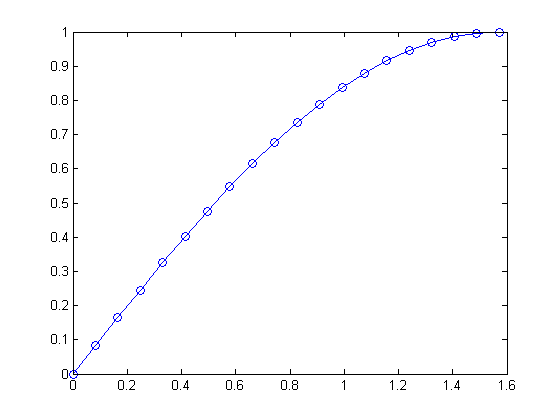
\includegraphics[scale=.5]{plot5.png}
\subsubsection*{100 Data Points [0, $\frac{\pi}{2}$]}
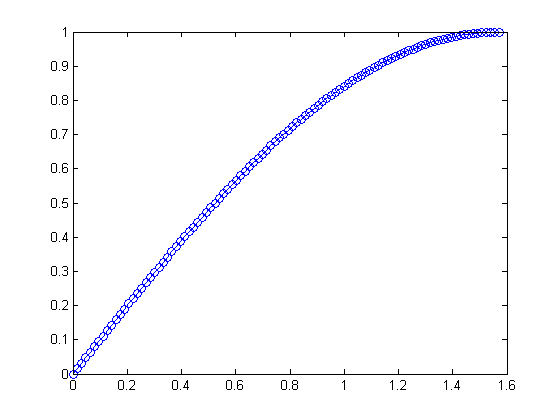
\includegraphics[scale=.5]{plot6.png}

\subsection*{best fit quadratic polynomial}
\begin{verbatim}
function [B,C, y2] = qfit()

n = 100;

x = linspace(-10,10,n)';
one = ones(size(x));
x2 = x.^2;

A = [one x x2];

B = A'*A;

y = x2*rand + x*rand + rand*one + .5*randn(size(x));

C =inv(B)*(A'*y);

y2 = x2*C(3)+x*C(2)+C(1);

plot(x , y, 'o-', x, y2, '-r' );

end
\end{verbatim}
\subsubsection*{20 Data Points}

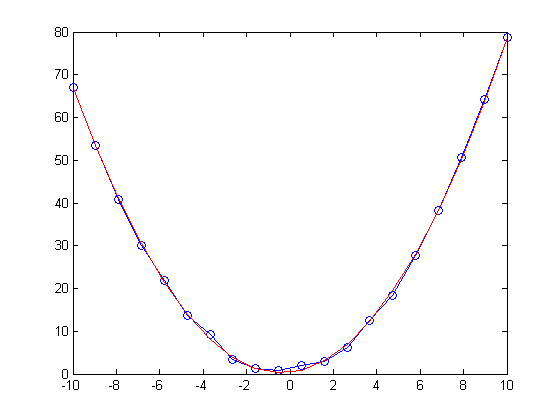
\includegraphics[scale=.5]{plot1.png}
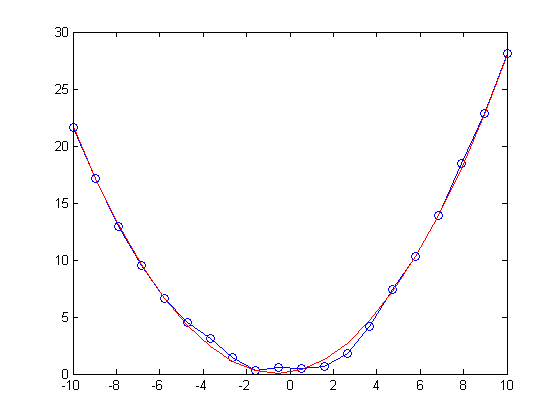
\includegraphics[scale=.5]{plot2.png}

\subsubsection*{100 Data Points}

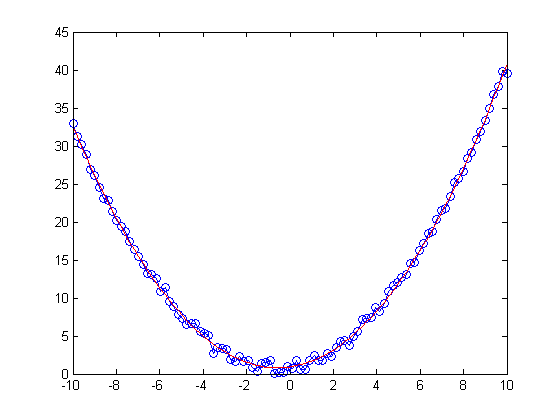
\includegraphics[scale=.5]{plot3.png}
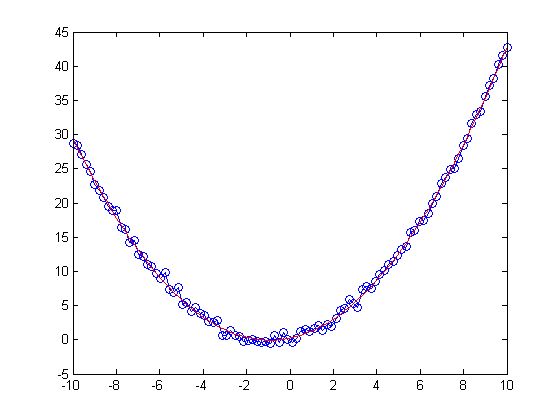
\includegraphics[scale=.5]{plot4.png}

\subsection*{Quadratic approximation for $\sin(x)$}
\begin{verbatim}
function sin()

n = 100;

x = linspace(0,pi/2,n)';
one = ones(size(x));
x2 = x.^2;

A = [one x x2];

B = A'*A;

y = sin(x) + .08*randn(size(x)); %noise added with randn

C =inv(B)*(A'*y);

y2 = x2*C(3)+x*C(2)+C(1);

figure
plot(x , y, 'o-', x ,y2, '-r');

end
\end{verbatim}

\begin{figure}[H]
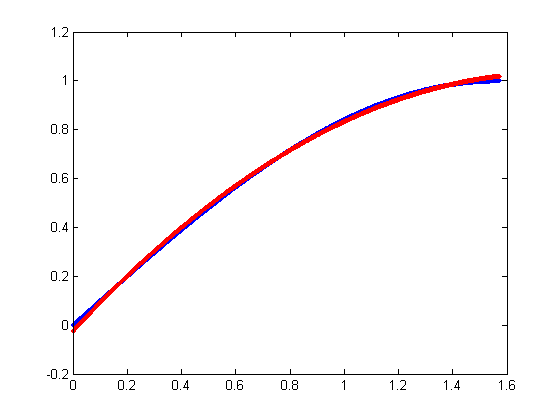
\includegraphics[scale=.8]{plot11.png}
\caption{Red = Quadratic Fit,  Blue is continuous sine function}
\end{figure}


\subsubsection*{With out Noise}
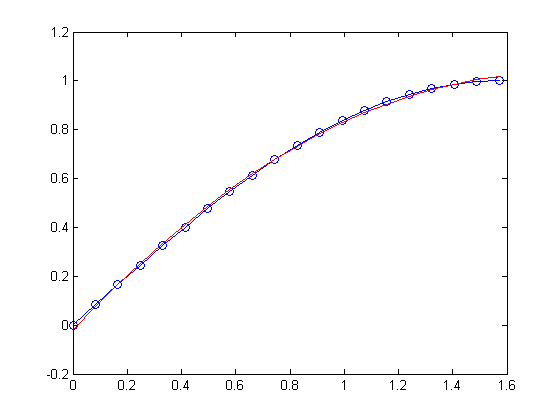
\includegraphics[scale=.5]{plot8.png}
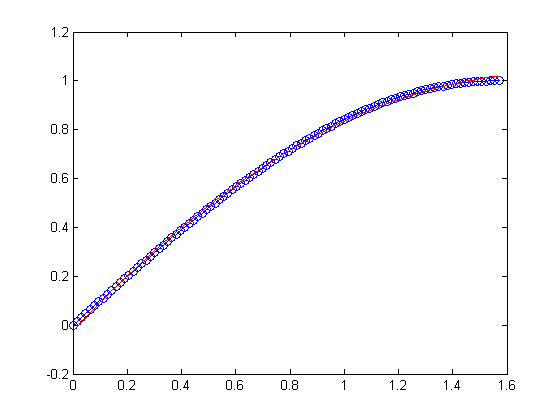
\includegraphics[scale=.5]{plot7.png}
\subsubsection*{With Normally Distributed Noise}
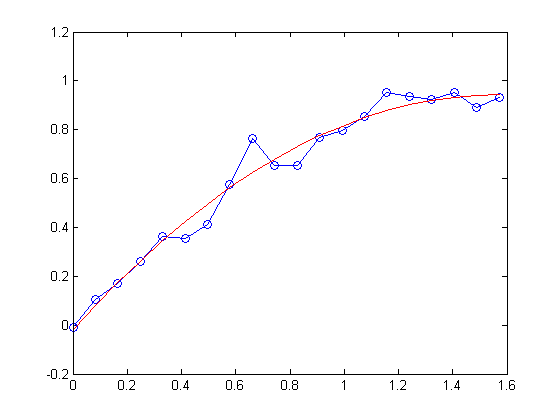
\includegraphics[scale=.5]{plot9.png}
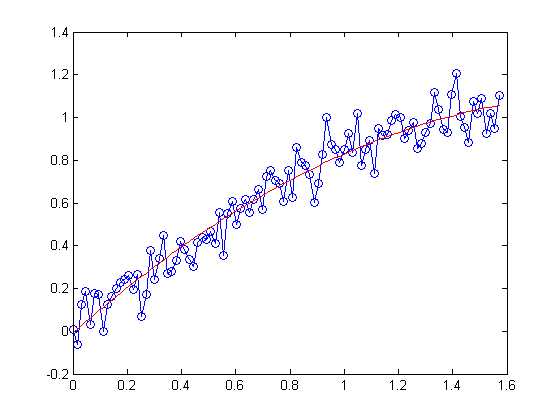
\includegraphics[scale=.5]{plot10.png}


\end{document}
